%%%%%%%%%%%%%%%%%%%%%%%%%%%%%%%%%%%%%%%%%%%%%%%%%%%%%%%%%%%%%%%%%%%%%%
% Lớp 10 | Phương pháp tọa độ trong mặt phẳng (𝑂𝑥𝑦) | Đường tròn trong mặt phẳng tọa độ
% Dạng 0H9?4-2: Phương trình đường tròn
% Số câu: 37  (sinh tự động bởi tach_cau.py; từ nay thầy sửa trực tiếp file này)
%%%%%%%%%%%%%%%%%%%%%%%%%%%%%%%%%%%%%%%%%%%%%%%%%%%%%%%%%%%%%%%%%%%%%%

%%%%%%%%%%%%%%%% TRẮC NGHIỆM 4 PHƯƠNG ÁN %%%%%%%%%%%%%%%%

% nguồn: MaHoaNH_TracNghiem_Lop10
\begin{ex}%[0H9N4-2]%[ma:26dc57f3]
	Phương trình  đường tròn tâm $I(2,-3)$ và đi qua điểm $M(-2,0)$ là
	\choice 
		{$(C):(x+2)^2+(y-3)^2=25$} 
		{$(C):(x-2)^2+(y+3)^2=5$} 
		 {$(C):(x+2)^2+(y-3)^2=5$}
		 {\True $(C):(x-2)^2+(y+3)^2=25$}
	\loigiai{ 
	Đường tròn tâm $I$ đi qua $M$ có bán kính $R=I  M=\sqrt{(-2-2)^2+(0+3)^2}=5$. \\Phương trình đường tròn cần tìm là $(C)\colon(x-2)^2+(y+3)^2=25$.}
\end{ex}

% nguồn: MaHoaNH_TracNghiem_Lop10
\begin{ex}%[0H9N4-2]%[ma:cc2204b5]
	Đường tròn tâm $I(a;b)$, bán kính bằng  $R$ có phương trình là
	 \choice
		 {$(x+a)^2+(y+b)^2=R$}
		{$(x-a)^2+(y-b)^2=R$} 
		{\True $(x-a)^2+(y-b)^2=R^2$} 
		{$(x+a)^2+(y+b)^2=R^2$} 
	\loigiai{ 
		Đường tròn tâm $I(a;b)$, bán kính bằng $R$  có phương trình là $(x-a)^2+(y-b)^2=R^2$.
	 }
\end{ex}

% nguồn: MaHoaNH_TracNghiem_Lop10
\begin{ex}%[0H9N4-2]%[ma:a2d1da64]
	Phương  trình nào sau đây là phương trình đường tròn
	\choice 
		 {$x^{2}+2y^{2}-4x-8y+1=0$}
		 {$4x^{2}+y^{2}-10x-6y-2=0$}
		{\True  $x^{2}+y^{2}-4x+6y-12=0$}
		 {$x^{2}+y^{2}-2x-8y+20=0$}
	\loigiai{ 
		Ta có  $x^{2}+y^{2}-4x+6y-12=0\Leftrightarrow(x-2)^2+(y+3)^2=5^2$.\\
		Vậy $x^{2}+y^{2}-4x+6y-12=0$  là phương trình đường tròn.
	 }
\end{ex}

% nguồn: MaHoaNH_TracNghiem_Lop10
\begin{ex}%[0H9H4-2]%[ma:d9cc8b12]
	Trong mặt phẳng $Oxy$, cho hai điểm $A(1;1)$, $B(7;5)$. Phương trình đường tròn đường  kính $AB$ là
	\choice 
		 {$x^2+y^2+8x+6y+12=0$}
		 {\True $x^2+y^2-8x-6y+12=0$}
		 {$x^2+y^2-8x-6y-12=0$}
		 {$x^2+y^2+8x+6y-12=0$}
	\loigiai{Đường tròn có tâm $I(4;3)$ là trung điểm của đoạn $AB$; bán kính $R=\dfrac{AB}{2}=\sqrt{13}$ có phương trình là 
	 $$(x-4)^2+(y-3)^2=13\Leftrightarrow x^2+y^2-8x-6y+12=0.$$}
\end{ex}

% nguồn: MaHoaNH_TracNghiem_Lop10
\begin{ex}%[0H9H4-2]%[ma:31d22279]
	Trong mặt  phẳng $Oxy$, phương trình nào sau đây là phương trình đường tròn?
	\choice 
		{$x^2+y^2-x-y+9=0$} 
		 {\True $x^2+y^2-x=0$}
		{$x^2+y^2-2xy-1=0$} 
		{$x^2-y^2-2x+3y-1=0$} 
	\loigiai{ 
		Xét phương trình $x^2+y^2-x=0$ có  $a=\dfrac{1}{2}$, $b=0$, $c=0\Rightarrow a^2+b^2-c > 0$ nên đây là phương trình của một đường tròn.
	} 
\end{ex}

% nguồn: MaHoaNH_TracNghiem_Lop10
\begin{ex}%[0H9H4-2]%[ma:8efee217]
	Trong mặt phẳng $Oxy$, đường tròn tâm $I(3;-1)$ và bán kính  $R=2$ có phương trình là
	 \choice
		 {$(x+3)^2+(y-1)^2=4$}
		 {$(x-3)^2+(y-1)^2=4$}
		 {\True $(x-3)^2+(y+1)^2=4$}
		 {$(x+3)^2+(y+1)^2=4$}
	\loigiai{ 
		Phương trình đường tròn có tâm $I(3;-1)$, bán kính $R=2$ là  $(x-3)^2+(y+1)^2=4$.
	} 
\end{ex}

% nguồn: MaHoaNH_TracNghiem_Lop10
\begin{ex}%[0H9H4-2]%[ma:5b2593b1]
	Đường tròn  tâm $I(-1; 2)$ và đi qua điểm $M(2; 1)$ có phương trình là
	\choice 
		{\True  $x^2+y^2+2x-4y-5=0$}
		{$x^2+y^2+2x-4y-3=0$} 
		{$x^2+y^2-2x-4y-5=0$} 
		 {$x^2+y^2+2x+4y-5=0$}
	\loigiai{Đường tròn có tâm $I(-1; 2)$ và đi  qua $M(2; 1)$ thì có bán kính là
		 $R=IM=\sqrt{3^2+(-1)^2}=\sqrt{10}$.\\
		Khi đó có phương trình  là $(x+1)^2+(y-2)^2=10\Leftrightarrow x^2+y^2+2x-4y-5=0$.
	} 
\end{ex}

% nguồn: MaHoaNH_TracNghiem_Lop10
\begin{ex}%[0H9H4-2]%[ma:590043ae]
	Trong mặt phẳng  tọa độ $Oxy$, viết phương trình của đường tròn có tâm là gốc tọa độ $O$ và tiếp xúc với đường thẳng $\Delta\colon x+y-2=0$.
	 \choice
		{\True  $x^2+y^2=2$}
		 {$x^2+y^2=\sqrt{2}$}
		{$(x-1)^2+(y-1)^2=2$} 
		{$x^2+y^2=4$} 
	\loigiai{ 
		Vì đường  tròn tâm $O$ tiếp xúc với $\Delta$ nên ta có $$R = \mathrm{d}(O;\Delta) = \dfrac{\left|-2\right|}{\sqrt{2}}=\sqrt{2}.$$
		Vậy phương trình đường tròn là $x^2+y^2=2$. 
	 }
\end{ex}

% nguồn: MaHoaNH_TracNghiem_Lop10
\begin{ex}%[0H9H4-2]%[ma:ff8c38c2]
	Trong mặt phẳng $Oxy$, đường tròn $(C)$ tâm $I(4;3)$ và tiếp xúc với đườngthẳng $\Delta \colon 3x-4y+5=0$ có phương trình là 
	 \choice
		 {$(x+4)^2+(y-3)^2=1$}
		{\True  $(x-4)^2+(y-3)^2=1$}
		 {$(x+4)^2+(y+3)^2=1$}
		{$(x-4)^2+(y+3)^2=1$} 
	\loigiai{ 
		$(C)$ có bán kính $R=\mathrm{d}\left(I,\Delta \right)=\dfrac{\left|3\cdot  4-4\cdot 3+5\right|}{\sqrt{3^2+\left(-4\right)^2}}=1$.\\
		Do đó,  $(C)$ có phương trình $(x-4)^2+(y-3)^2=1$.
	} 
\end{ex}

% nguồn: MaHoaNH_TracNghiem_Lop10
\begin{ex}%[0H9H4-2]%[ma:246a338a]
	Trong mặt phẳng toạ độ $Oxy$, phương trình đường tròn nhận $AB$ làm đường kính biết $A(-3;2)$ và $B(3;-4)$ là 
	 \choice
		{$(x+1)^2+y^2=9$} 
		 {$(x+1)^2+y^2=18$}
		{$x^2+(y+1)^2=9$} 
		{\True $x^2+(y+1)^2=18$} 
	 \loigiai{
		Gọi $I$ là tâm của đường tròn khi đó $I(0;-1)$ và $AB=\sqrt{6^2+6^2}=6\sqrt{2}$. Suy ra  $R=3\sqrt{2}$.\\
		Vậy đường tròn có phương trình  là $x^2+(y+1)^2=18$.
	 }
\end{ex}

% nguồn: MaHoaNH_TracNghiem_Lop10
\begin{ex}%[0H9H4-2]%[ma:c8c0d31a]
	Trong mặt  phẳng $Oxy$, đường tròn $(C)$ tiếp xúc với trục tung tại điểm $A(0;-2)$ và đi qua điểm $B(4;-2)$ có phương trình là
	\choice 
		{\True $(x-2)^2+(y+2)^2=4$} 
		 {$(x+2)^2+(y-2)^2=4$}
		{$(x-3)^2+(y-2)^2=4$} 
		{$(x-3)^2+(y+2)^2=4$} 
	\loigiai{ 
		Vì  $y_A=y_B=-2$ nên $ AB\perp y'Oy$ và $AB$ là đường kính của $(C)$.\\
		Suy  ra $I(2;-2)$ và bán kính $R=IA=2$.\\
		Vậy  $(C)\colon (x-2)^2+(y+2)^2=4$.
	} 
\end{ex}

% nguồn: MaHoaNH_TracNghiem_Lop10
\begin{ex}%[0H9H4-2]%[ma:2726f832]
	Trong hệ trục $Oxy$, cho hai điểm $A(-1;-3)$, $B(-3; 5)$, phương trình đường tròn có đường kính $AB$ là 
	 \choice
		{\True  $(x+2)^2+(y-1)^2=17$}
		 {$(x+2)^2+(y-1)^2=\sqrt{17}$}
		{$(x+1)^2+(y-4)^2=\sqrt{68}$} 
		 {$(x+1)^2+(y+3)^2=68$}
	 \loigiai{
		Gọi $I$ là  tâm của đường tròn.\\
		Ta  có $I$ là trung điểm của $AB\Rightarrow$ là $I(-2; 1)$, $\overrightarrow{AI}=(-1; 4)$.\\
		Bán kính của  đường tròn là $R=AI=\sqrt{(-1)^2+4^2}=\sqrt{17}$.\\
	Vậy  phương trình của đường tròn là $(x+2)^2+(y-1)^2=17$.}
\end{ex}

% nguồn: MaHoaNH_TracNghiem_Lop10
\begin{ex}%[0H9H4-2]%[ma:b6f1aa61]
	Trong mặt phẳng $Oxy$, cho hai điểm  $A(5;-1)$, $B(-3;7)$. Đường tròn có đường kính $AB$ có phương trình là
	 \choice
		{\True $x^2+y^2-2x-6y-22=0$} 
		 {$x^2+y^2-2x-6y+22=0$}
		 {$x^2+y^2-2x-y+1=0$}
		 {$x^2+y^2+6x+5y+1=0$}
	 \loigiai{
		Tâm $I$ của đường tròn là trung điểm $AB$ nên $I(1;3)$.\\ 
		Bán  kính $R=\dfrac{1}{2} AB=\dfrac{1}{2} \sqrt{\left(-3-5\right)^2+\left(7+1\right)^2}=4\sqrt{2}$.\\
		Vậy  phương trình đường tròn là $(x-1)^2+(y-3)^2=32\Leftrightarrow x^2+y^2-2x-6y-22=0$.
	} 
\end{ex}

% nguồn: MaHoaNH_TracNghiem_Lop10
\begin{ex}%[0H9H4-2]%[ma:b1ff2bda]
	Trong mặt phẳng $Oxy$, cho hai điểm $A(-2;1)$, $B(3;5)$. Tập hợp điểm $M(x;y)$ nhìn $AB$ dưới một góc vuông  nằm trên đường tròn có phương trình là
	 \choice
		{\True $x^2+y^2-x-6y-1=0$} 
		 {$x^2+y^2+x+6y-1=0$}
		{$x^2+y^2+5x-4y+11=0$} 
		{Chọn khác} 
	 \loigiai{
		Tập hợp điểm $M(x;y)$ nhìn $AB$ dưới một góc vuông là đường tròn  đường kính $AB$ và tâm là trung điểm của $AB$.\\
		Trung điểm của $AB$ là $I\left(\dfrac{1}{2};3\right)$.\\ 
		Bán kính đường  tròn là $R=\dfrac{AB}{2}=\dfrac{\sqrt{5^2+4^2}}{2}=\dfrac{\sqrt{41}}{2}$.\\
		Phương trình đường tròn $\left(x-\dfrac{1}{2}  \right)^2+(y-3)^2=\dfrac{41}{4}$ $\Leftrightarrow x^2+y^2-x-6y-1=0$.
	} 
\end{ex}

% nguồn: MaHoaNH_TracNghiem_Lop10
\begin{ex}%[0H9H4-2]%[ma:cf821717]
	Trong mặt phẳng $Oxy$, tâm  của đường tròn qua ba điểm $A(2;1)$, $B(2; 5)$, $C(-2; 1)$ thuộc đường thẳng có phương trình
	 \choice
		{\True $x-y+3=0$} 
		 {$x-y-3=0$}
		{$-x+y+3=0$} 
		{$x+y+3=0$} 
	\loigiai{ 
		Phương trình $(C)$ có dạng $x^2+y^2-2ax-2by+c=0, (a^2+b^2+c > 0)$. Tâm $I(a; b)$.\\ 
		 \[
		\heva {& A(2;1)\in (C) \\ & B(2; 5)\in (C)  \\ & C(-2; 1)\in (C)} \Leftrightarrow \heva{& 4+1-4a-2b+c=0 \\ & {4+25-4a-10b+c=0} \\ & {4+1+4a-2b+c=0}} \Leftrightarrow \heva{& {a=0} \\ & {b=3} \\ & {c=1} } \Rightarrow I(0; 3).
		 \]
		Lần lượt thế tọa độ $I$ vào các phương  trình để kiểm tra.
	 }
\end{ex}

% nguồn: MaHoaNH_TracNghiem_Lop10
\begin{ex}%[0H9H4-2]%[ma:8e0f6cd1]
	Trong mặt phẳng $Oxy$, viết phương trình đường tròn đi  qua ba điểm $A(0;4)$, $B(2;4)$, $C(2;0)$.
	 \choice
		 {$x^{2}+y^{2}+2x-4y=0$}
		 {$x^{2}+y^{2}-2x+4y=0$}
		{$x^{2}+y^{2}+2x+4y=0$} 
		{\True  $x^{2}+y^{2}-2x-4y=0$}
	 \loigiai{
		Giả sử phương  trình đường tròn đi qua $3$ điểm $A$, $B$, $C$ có dạng
		 $(C)\colon x^{2}+y^{2}+2ax+2by+c=0$.\\
		Thay tọa độ  $3$ điểm $A(0;4)$, $B(2;4)$, $C(2;0)$, ta được
		$\heva{&8b+c=-164\\&a+8b+c=-204\\&a+c=-4}\Leftrightarrow\heva{&a=-1\\&b=-2\\&c=0.}$\\ 
		Vậy  $(C)\colon x^{2}+y^{2}-2x-4y=0$.
	} 
\end{ex}

% nguồn: MaHoaNH_TracNghiem_Lop10
\begin{ex}%[0H9H4-2]%[ma:b6b74eca]
	 Trong hệ trục $Oxy$, cho hai điểm $A(-1;-3)$, $B(-3;5)$. Phương trình đường tròn có đường kính $AB$ là
	\choice 
		{\True  $(x+2)^2+(y-1)^2=17$}
		 {$(x+2)^2+(y-1)^2=\sqrt{17}$}
		 {$(x+1)^2+(y-4)^2=\sqrt{68}$}
		 {$(x+1)^2+(y+3)^2=68$}
	\loigiai{ 
		Gọi $I$ là trung điểm của $AB$,  ta có
		\[I = \left(\dfrac{-1+(-3)}{2};  \dfrac{-3+5}{2} \right) = (-2;1).\]
		Bán kính của đường  tròn là
		\[R = AI  = \sqrt{(-1+2)^2+( -3-1)^2} = \sqrt{1+16} = \sqrt{17}.\]
		Vậy phương trình  của đường tròn là
		\[(x+2)^2+(y-1)^2=17.\] 
	} 
\end{ex}

% nguồn: MaHoaNH_TracNghiem_Lop10
\begin{ex}%[0H9H4-2]%[ma:13cd789d]
	Trong mặt phẳng $Oxy$, đường tròn $(C)$ đi qua hai điểm $A(1;3)$, $B(3;1)$ và  có tâm nằm trên đường thẳng $d\colon 2x-y+7=0$ có phương trình là
	\choice 
		{$(x-7)^2+(y-7)^2=102$} 
		{\True $(x+7)^2+(y+7)^2=164$} 
		 {$(x-3)^2+(y-5)^2=25$}
		 {$(x+3)^2+(y+5)^2=25$}
	\loigiai{ 
		$I(a;b)$ là tâm của đường tròn  $(C)$, do đó
		\[ 
		AI^2=BI^2 \Rightarrow (a-1)^2+(b-3)^2=(a-3)^2+(b-1)^2. 
		 \]
		Suy ra $a=b\; \; (1)$. Mà $I(a; b)\in d\colon 2x-y+7=0$ nên $ 2a-b+7=0\;  \; (2)$.\\
		Thay (1) vào  (2) ta có $a=-7\Rightarrow b=-7\Rightarrow R^2=AI^2=164$.\\
		 Vậy $(C)\colon (x+7)^2+(y+7)^2=164$.
	} 
\end{ex}

% nguồn: MaHoaNH_TracNghiem_Lop10
\begin{ex}%[0H9H4-2]%[ma:a6b70240]
	Trong mặt phẳng $Oxy$,  đường tròn đi qua $3$ điểm $A(0;2)$, $B(2;2)$, $C(1;1+\sqrt{2})$ có phương trình là
	 \choice
		 {$x^2+y^2+2x+2y-\sqrt{2}=0$}
		{\True $x^2+y^2-2x-2y=0$} 
		 {$x^2+y^2-2x-2y-2=0$}
		{$x^2+y^2+2x-2y+\sqrt{2}=0$} 
	\loigiai{ 
		Gọi phương trình đường tròn cần tìm có dạng $x^2+y^2-2ax-2by+c=0\left(a^2+b^2-c > 0\right)$.\\ 
		Đường tròn đi qua $3$  điểm $A(0;2)$, $B(2;2)$, $C(1;1+\sqrt{2})$ nên ta có
		\[ 
		\heva{& 4-4b+c=0 \\ & 8-4a-4b+c=0 \\ & 4+2\sqrt{2}-2a-2\left(1+\sqrt{2} \right)b+c=0.} 
		\Leftrightarrow \heva{& a=1 \\ & b=1 \\ &  c=0.}
		\] 
		Vậy phương trình đường tròn  đi qua $3$ điểm $A(0;2)$, $B(2;2)$, $C(1;1+\sqrt{2})$ là
		\[ 
		x^2+y^2-2x-2y=0. 
		 \]
	} 
\end{ex}

% nguồn: MaHoaNH_TracNghiem_Lop10
\begin{ex}%[0H9H4-2]%[ma:c21aff27]
	Phương trình $x^2+y^2-2(m+1)x-2(m+2)y+6m+7=0$ là phương trình đường tròn khi  và chỉ khi
	 \choice
		{$m <  0$}
		{$m  < 1$}
		{$m  > 1$}
		{\True  $m <-1$ hoặc $m > 1$}
	\loigiai{ 
		 Ta có
		\begin{eqnarray*}
			 & & x^2+y^2-2(m+1)x-2(m+2)y+6m+7=0\\
			&  \Leftrightarrow & x^2-2(m+1)x+(m+1)^2+y^2-2(m+2)y+(m+2)^2 = (m+1)^2-(m+2)^2 - 6m- 7\\
			& \Leftrightarrow &  \left[x-(m+1)\right]^2+\left[y-(m+2)\right]^2=2m^2-2.
		\end{eqnarray*}
		Vậy điều kiện  để phương trình đã cho là phương trình đường tròn là
		 \[
		2m^2-2> 0\Leftrightarrow \hoac{& m <-1 \\ & m > 1.} 
		\] 
	} 
\end{ex}

% nguồn: MaHoaNH_TracNghiem_Lop10
\begin{ex}%[0H9H4-2]%[ma:15f72ca2]
	Phương trình nào sau  đây là phương trình của đường tròn?
	\begin{itemize}
		\item[(1)] $x^2+y^2-4x+15y-12=0$. 
		\item[(2)] $x^2+y^2-3x+4y+20=0$. 
		\item[(3)] $2x^2+2y^2-4x+6y+1=0$. 
	\end{itemize}
	 \choice
		 {$(1)$}
		{$(2)$} 
		 {$(3)$}
		{\True  $(1)$ và $(3)$}
	 \loigiai{
		\begin{itemize}
			\item $(1)$ ta  có $a^2+b^2-c=4+\left(\dfrac{15}{2} \right)^2+12=\dfrac{289}{4} > 0$.
			\item  $(2)$ ta có $a^2+b^2-c=\left(\dfrac{3}{2} \right)^2+\left(\dfrac{4}{2} \right)^2-20=-\dfrac{55}{4} < 0$.
			\item $(3)  \Leftrightarrow x^2+y^2-2x-3y+\dfrac{1}{2}=0$.\\
			Phương trình  này có $a^2+b^2-c=1+\left(\dfrac{3}{2} \right)^2-\dfrac{1}{2}=\dfrac{11}{4} > 0$.
		\end{itemize}
		Vậy chỉ $(1)$  và $(3)$ là phương trình đường tròn.
	 }
\end{ex}

% nguồn: MaHoaNH_TracNghiem_Lop10
\begin{ex}%[0H9V4-2]%[ma:4248b5c2]
	Trong mặt  phẳng $Oxy$, đường tròn $(C)$ đi qua điểm $A(2;4)$ và tiếp xúc với các trục tọa độ có phương trình là
	 \choice
		{\True  $(x-2)^2+(y-2)^2=4$ hoặc $(x-10)^2+(y-10)^2=100$}
		{$(x+2)^2+(y+2)^2=4$  hoặc $(x-10)^2+(y-10)^2=100$}
		{$(x+2)^2+(y+2)^2=4$ hoặc  $(x+10)^2+(y+10)^2=100$}
		{$(x-2)^2+(y-2)^2=4$ hoặc $(x+10)^2+(y+10)^2=100$} 
	 \loigiai{
		Ta có $(C)\colon  (x-a)^2+(y-b)^2=R^2$ tiếp xúc với các trục tọa độ nên $\left|a\right|=\left|b\right|=R$ và điểm $A(2;4)\in (C)$ nằm trong góc phần tư thứ nhất nên $I(a;b)$ cũng ở góc phần tư thứ nhất. \\
		Suy  ra $a=b=R$. Vậy $(C)\colon (x-a)^2+(y-a)^2=a^2$.\\
		Khi  đó
		 \[
		A\in (C)\Rightarrow  (2-a)^2+(4-a)^2=a^2\Leftrightarrow a^2-12a+20=0\Leftrightarrow
		\hoac{& a=2  \\ & a=10.}
		 \]
		Vậy phương trình  các đường tròn là $(x-2)^2+(y-2)^2=4$ hoặc $(x-10)^2+(y-10)^2=100$.
	 }
\end{ex}

% nguồn: MaHoaNH_TracNghiem_Lop10
\begin{ex}%[0H9V4-2]%[ma:f71f9045]
	Trong mặt phẳng $(Oxy)$, đường tròn đi qua ba điểm $A(1;2)$, $B(5;2)$, $C(1;-3)$ có phương  trình là
	 \choice
		 {$x^2+y^2+6x+y-1=0$}
		 {$x^2+y^2-6x-y-1=0$}
		{\True  $x^2+y^2-6x+y-1=0$}
		{$x^2+y^2+6x-y-1=0$} 
	 \loigiai{
		Phương trình đường tròn dạng  khai triển $x^2+y^2-2ax-2by+c=0$.\\
		Do đường tròn đi qua  ba điểm $A(1;2)$, $B(5;2)$, $C(1;-3)$ nên
		\allowdisplaybreaks 
		\begin{eqnarray*}
			 &&\heva{&1+4-2a-4b+c=0\\&25+4-10a-4b+c=0\\&1+9-2a+6b+c=0}\\
			 &\Leftrightarrow&\heva{&-2a-4b+c=-5\\&-10a-4b+c=-29\\&-2a+6b+c=-10}\\
			&\Leftrightarrow&\heva{&a=3\\&b=-\dfrac{1}{2}\\&c=-1.} 
		\end{eqnarray*}
		Vậy phương  trình đường tròn là $x^2+y^2-6x+y-1=0$.
	} 
\end{ex}


%%%%%%%%%%%%%%%% ĐÚNG/SAI %%%%%%%%%%%%%%%%

% nguồn: MaHoaNH_DungSai_Lop10
\begin{ex}%[0H9N4-2]%[ma:f8837aa9]
	 Trong các khẳng định sau đây, khẳng định nào đúng, khẳng định nào sai?
	 \choiceTF
		{\True  Đường tròn tâm $O(0;0)$, bán kính $R=2$ có phương trình là $x^2+y^2=4$}
		{Đường tròn tâm $I(1;-1)$  và đi qua điểm $A(1;2)$ có phương trình là $(x+1)^2+(y-1)^2=9$}
		{\True Đường tròn đường kính $BC$ với $B(1;-2)$, $C(5;2)$ có phương trình  là $(x-3)^2+y^2=8$}
		{\True Đường tròn tâm $J(0;-2)$ và tiếp xúc với đường thẳng $\Delta \colon  x+y-2=0$ có phương trình là $x^2+(y+2)^2=8$}
	\loigiai{ 
		\begin{itemchoice}
			\itemch Đường tròn tâm $O(0;0)$, bán kính $R=2$  có phương trình là $x^2+y^2=4$
			\itemch Đường tròn tâm $I(1;-1)$ và đi qua điểm $A(1;2)$ có bán kính $R=IA=\sqrt{(1-1)^2+(2+1)^2}=3$ nên có phương  trình là $(x-1)^2+(y+1)^2=9$.
			\itemch Đường tròn đường kính $BC$ với $B(1;-2)$, $C(5;2)$ có tâm $K(3;0)$ là trung điểm của $BC$,  bán kính $R=KC=\sqrt{(5-3)^2+2^2}=2\sqrt{2}$ nên có phương trình là $(x-3)^2+y^2=8$.
			\itemch Đường tròn tâm $J(0;-2)$ và tiếp xúc với đường thẳng  $\Delta \colon x+y-2=0$ có bán kính $$R=\mathrm{d}(J,\Delta) = \dfrac{|0-2-2|}{\sqrt{1^2+1^2}}=2\sqrt{2}$$ nên có phương trình là $x^2+(y+2)^2=8$.
		\end{itemchoice}
	} 
\end{ex}

% nguồn: MaHoaNH_DungSai_Lop10
\begin{ex}%[0H9H4-2]%[ma:a8c892aa]
	Trong  mặt phẳng $Oxy$, cho đường tròn $(C)$ đi qua hai điểm $A(2;3)$, $B(-1;1)$ và có tâm thuộc đường thẳng $\Delta\colon x-3y-11=0$.
	\choiceTF 
		{$(C)$  có tâm $I\left(7;-\dfrac{4}{3}\right)$}
		{\True Điểm $O(0;0)$ nằm bên trong  đường tròn $(C)$}
		{Đường kính của $(C)$ bằng  $65$}
		{\True Đường  tròn $(C)$ đi qua điểm $N(0;2)$}
	\loigiai{ 
		\begin{itemchoice}
			\itemch {\bf Sai.} Gọi tâm đường tròn là $I(3t+11;t) \in \Delta$.  Ta có $$IA^2=IB^2
			\Leftrightarrow (3t+11-2)^2+(t-3)^2=(3t+11-2)^2+(t-1)^2\Leftrightarrow  t=-\dfrac{5}{2}.$$
			 Suy ra $I\left(\dfrac{7}{2};-\dfrac{5}{2}\right)$.
			\itemch {\bf  Đúng.} Bán kính $R=IA=\sqrt{\left(2-\dfrac{7}{2}\right)^2+\left(3+\dfrac{5}{2}\right)^2}=\sqrt{\dfrac{65}{2}}$. \\
			$IO<R$ nên điểm $O(0;0)$ nằm bên trong  đường tròn $(C)$.
			\itemch {\bf Sai.} Đường  kính $2R=\sqrt{130}$.
			\itemch {\bf Đúng.} Phương  trình đường tròn $(C)$ là $\left(x-\dfrac{7}{2}\right)^2+\left(y+\dfrac{5}{2}\right)^2=\dfrac{65}{2}$. \\
			Đường tròn $(C)$ đi  qua điểm $N(0;2)$
		\end{itemchoice}
	} 
\end{ex}

% nguồn: MaHoaNH_DungSai_Lop10
\begin{ex}%[0H9H4-2]%[ma:122adae1]
	Trong mặt phẳng $Oxy$, cho đường tròn $(C)$ đi qua hai điểm $A(2;3)$, $B(-1;1)$ có tâm thuộc $\Delta  \colon x-3y-11=0$.
	 \choiceTF
		{Tâm của đường tròn $(C)$ là $I\left(7;  -\dfrac{4}{3}\right)$}
		{\True Điểm $O(0;0)$ nằm  bên trong đường tròn $(C)$}
		{ Đường kính của đường tròn $(C)$ bằng $65$} 
		{\True Đường tròn $(C)$ đi qua  điểm $(0;2)$}
	 \loigiai{
		\begin{itemchoice}
			\itemch Gọi tâm  đường tròn là $I(3t+11;t)\in \Delta$. Ta có $IA=IB\Leftrightarrow IA^2=IB^2$.
			\[ 
			\Leftrightarrow (3t+11-2)^2+(t-3)^2=(3t+11+1)^2+(t-1)^2\Leftrightarrow 22t=-55\Leftrightarrow  t=-\dfrac{5}{2}.
			 \]
			Suy ra  $I\left(\dfrac{7}{2};-\dfrac{5}{2} \right)$.
			\itemch Ta có $OI^2  = \dfrac{49}{4} + \dfrac{25}{4} = \dfrac{74}{4} < R^2 = \dfrac{130}{4}$. Suy ra điểm $O$ nằm bên trong đường tròn.
			\itemch Bán kính đường tròn  $R=IA=\sqrt{\left(2-\dfrac{7}{2} \right)^2+\left(3+\dfrac{5}{2} \right)^2}=\dfrac{\sqrt{130}}{2}$.\\
			Suy ra  đường kính là $d = 2R = \sqrt{130}$.
			\itemch Phương trình đường  tròn $(C)\colon \left(x-\dfrac{7}{2} \right)^2+\left(y+\dfrac{5}{2} \right)^2=\dfrac{65}{2}$.\\
			 Thay tọa độ điểm $A(0;2)$ ta thấy thỏa mãn.
		\end{itemchoice}
	 }
\end{ex}

% nguồn: MaHoaNH_DungSai_Lop10
\begin{ex}%[0H9H4-2]%[ma:7e43d000]
	Trong mặt  phẳng $Oxy$, cho ba điểm $A(2;-1)$, $B(4;3)$, $C(-5;0)$.
	Xét tính đúng, sai của mỗi khẳng  định sau.
	\choiceTF 
		{\True $\vec{AC}(-7;  1)$}
		{\True Phương trình đường thẳng $AC\colon  x+7y+5=0$}
		{Khoảng cách từ $B$ đến đường thẳng  $AC$ bằng $2\sqrt{2}$}
		{Đường tròn  tâm $B$ tiếp xúc với đường thẳng $AC$ có phương trình $(x-4)^2+(y-3)^2=8$}
	\loigiai{ \begin{enumerate}
		\item  Ta có
		$\overrightarrow{AC}=(-7;1)$. 
		\item Đường thẳng đi qua hai điểm $AC$ có véc-tơ chỉ phương $\overrightarrow{AC}=(-7;1)$. Suy ra đường thẳng này có véc-tơ pháp tuyến $\overrightarrow{n}=(1;7)$ và đi qua điểm $A(2;-1)$  nên có phương trình
		\[1(x-2)+7(y+1)=0\Leftrightarrow  x+7y+5=0.\]
		\item  Khoảng cách từ $B$ đến đường thẳng $AC$ là
		 \[h=\mathrm{d}\left(B, AC\right)=\dfrac{|4+7\cdot 3+5|}{\sqrt{1^2+7^2}}=3\sqrt{2}.\]
		 \item Đường tròn tâm $B(4;3)$ tiếp xúc với đường thẳng $AC$ nên có
		bán kính 
		 $R=h=3\sqrt{2}$.\\
		 Phương trình đường tròn có tâm $B(4;3)$, bán kính $R=3\sqrt{2}$ là
		 \[(x-4)^2+(y-3)^2=18.\]
	\end{enumerate}
} 
\end{ex}

% nguồn: MaHoaNH_DungSai_Lop10
\begin{ex}%[0H9H4-2]%[ma:1fe9a065]
	Xác  định tính đúng, sai của các khẳng định sau
	 \choiceTF
		{\True Phương trình đường tròn có tâm $I(-2;-5)$ và bán kính  $R=8$ là $(x+2)^2+(y+5)^2=64$}
		{Phương trình đường tròn có tâm $I(-1; 3)$ và tiếp xúc với đường thẳng $\Delta: x+2 y+5=0$ là $(x+1)^2+(y-3)^2=30$} 
		{Phương trình đường tròn có tâm $I(-3; 2)$ và đi qua điểm $A(-4; 1)$  là $(x+3)^2+(y-2)^2=20$}
		{\True Phương trình đường tròn đi qua ba  điểm $A(5;-2)$, $B(3; 0)$, $C(-1; 2)$ là $(x+4)^2+(y+9)^2=130$}
	 \loigiai{
		\begin{itemchoice}
			\itemch Phương trình đường tròn có tâm $I(-2;-5)$ và bán kính $R=8$ là \begin{center}
			$(x-(-2))^2+(y-(-5))^2=64$  hay $(x+2)^2+(y+5)^2=64$.
		\end{center}
		\itemch Bán kính đường  tròn là $R=d(I,\Delta)=\dfrac{\left|-1+2\cdot 3+5 \right|}{\sqrt{1^2+2^2}}=2\sqrt{5}$.\\
		Phương trình đường tròn có tâm $I(-1; 3)$ và tiếp xúc với đường thẳng $\Delta: x+2 y+5=0$ là  $$(x+1)^2+(y-3)^2=20.$$
		\itemch Bán kính đường tròn là  $R=IA=\sqrt{(-4-(-3))^2+(1-2)^2}=\sqrt{2}$.\\
		Phương trình đường tròn có tâm $I(-3; 2)$ và đi qua điểm $A(-4; 1)$  là $$(x+3)^2+(y-2)^2=2.$$
		\itemch Gọi $x^2+y^2-2ax-2by+c=0$ là phương trình đường tròn $(C)$ đi qua ba điểm $A(5;-2)$,  $B(3; 0)$, $C(-1; 2)$.\\
		Do $A$, $B$, $C$ thuộc đường tròn $(C)$ nên ta  có hệ phương trình
		\begin{eqnarray*}
			 &&\heva{&5^2+(-2)^2-10a+4b+c=0\\&3^2+0^2-6a+c=0\\&(-1)^2+2^2+2a-4b+c=0}\\
			&\Leftrightarrow  &\heva{&-10a+4b+c=-29\\&-6a+c=-9\\&2a-4b+c=-5}\\
			 &\Leftrightarrow &\heva{&a=-4\\&b=-9\\&c=-33}
		\end{eqnarray*}
		Ta  có $\sqrt{a^2+b^2-c}=\sqrt{(-4)^2+(-9)^2-(-33)}=\sqrt{130}$.\\
		Phương trình đường tròn đi qua ba điểm  $A(5;-2)$, $B(3; 0)$, $C(-1; 2)$ là $$(x+4)^2+(y+9)^2=130.$$
	\end{itemchoice}
} 
\end{ex}

% nguồn: MaHoaNH_DungSai_Lop10
\begin{ex}%[0H9H4-2]%[ma:4fcae3b1]
	 Trong các khẳng định sau đây, khẳng định nào đúng, khẳng định nào sai?
	 \choiceTF
		{Đường tròn có tâm nằm trên đường thẳng $\Delta\colon \heva{&x=1+t\\&y=2-t}$, đi qua điểm $P(1;0)$ và có bán kính $R=\sqrt{2}$ có phương  trình là $(x-1)^2+y^2=2$}
		{\True Đường tròn có tâm  nằm trên trục $Ox$ và tiếp xúc với đường thẳng $d\colon x-y+2=0$ tại điểm $A(1;3)$ có phương trình là $(x-4)^2+y^2=18$}
		{Đường tròn đi qua ba điểm $M(1;2)$,  $N(2;0)$ và $P(6;2)$ có phương trình $(x-3)^2+(y+2)^2=\dfrac{25}{4}$}
		 {\True Đường tròn có tâm $J$ nằm trên đường thẳng $a\colon x+y-3=0$ và đi qua hai điểm $B(1;4)$, $C(5;2)$ có phương trình là $(x-2)^2+(y-1)^2=10$}
	 \loigiai{
		\begin{itemchoice}
			\itemch Giả sử $I$ nằm trên $\Delta$ là  tâm đường tròn, ta có $I(1+t;2-t)$.\\
			Theo bài ra, ta có $PI=\sqrt{2} \Leftrightarrow \sqrt{t^2+(2-t)^2}=\sqrt{2} \Leftrightarrow 2t^2-4t+2=0 \Leftrightarrow t=1  \Rightarrow I(2;1)$.\\
			Vậy phương trình  đường tròn cần tìm là $(x-2)^2+(y-1)^2=2$.
			\itemch Đường tròn $(C)$ tiếp xúc với đường thẳng $d\colon x-y+2=0$ tại điểm $A(1;3)$ có tâm  nằm trên đường thẳng $d_1$ vuông góc với $d$ tại $A$.\\
			 Phương trình đường thẳng $d_1\colon (x-1)+(y-3)=0 \Leftrightarrow x+y-4=0$.\\
			Do tâm $I$ của $(C)$ nằm trên $Ox$ nên tọa độ tâm $I$ là nghiệm của  hệ phương trình $$\heva{&y=0\\&x+y-4=0} \Leftrightarrow \heva{&x=4\\&y=0} \Rightarrow I(4;0).$$
			Bán kính đường tròn là  $R=IA=\sqrt{(-3)^2+3^2}=3\sqrt{2}$.\\
			Phương trình  đường tròn là $(x-4)^2+y^2=18$.
			\itemch Giả sử đường tròn đi qua ba điểm $M$, $N$, $P$ có phương trình tổng  quát là
			$$x^2+y^2-2ax-2by+c=0 \,  (a^2+b^2>c)\quad (*)$$
			Khi đó ta  có hệ phương trình
			$$\heva{&-2a-4b+c=-5\\& -4a+c=-4\\&  -12a-4b+c=-40} \Leftrightarrow \heva{&a=\dfrac{7}{2}\\&b=2\\&c=10}$$
			thỏa mãn điều kiện $a^2+b^2>c$.\\ 
			Vậy phương trình đường tròn đi qua ba điểm $M$, $N$, $P$ là 
			$$x^2+y^2-7x-4y+10=0 \Leftrightarrow  \left(x-\dfrac{7}{2}\right)^2 + (y-2)^2=\dfrac{25}{4}.$$
			\itemch Đường tròn có tâm $J$ thuộc  đường thẳng $a\colon x+y-3=0$ nên có $J(m;3-m)$.\\
			Do đường  tròn đi qua hai điểm $B$ và $C$ nên $JB=JC\Leftrightarrow JB^2=JC^2$, do đó
			$$(1-m)^2+(1+m)^2=(5-m)^2+(m-1)^2  \Leftrightarrow m^2+2m+1=m^2-10m+25 \Leftrightarrow m=2.$$
			Suy ra $J(2;1)$, bán kính  đường tròn $R=JB=\sqrt{(1-2)^2+(4-1)^2}=\sqrt{10}$.\\
			Vậy phương trình đường tròn tâm $J$ nằm trên đường thẳng $a\colon x+y-3=0$ và đi qua hai điểm $B(1;4)$, $C(5;2)$ là  $(x-2)^2+(y-1)^2=10$.
		\end{itemchoice}
	} 
\end{ex}

% nguồn: MaHoaNH_DungSai_Lop10
\begin{ex}%[0H9H4-2]%[ma:3b7c20db]
	Trong mặt phẳng tọa độ $O x y$, cho đường thẳng $\Delta\colon 2 x-y+2=0$. Gọi $(C)$ là đường tròn có tâm $I(-2; 3)$ và  cắt đường thẳng $\Delta$ tại hai điểm phân biệt $A$, $B$ sao cho $A B=4$. Trong các khẳng định sau, khẳng định nào đúng, khẳng định nào sai?
	 \choiceTF
		{Đoạn thẳng $AB$ là  đường kính của đường tròn $(C)$}
		{\True Bán kính của đường tròn $(C)$  là $R=3$}
		{\True Đường tròn $(C)$ có phương trình là $(x+2)^2+(y-3)^2=9$} 
		{\True Diện tích tam giác $IAB$ là  $S=2\sqrt{5}$}
	 \loigiai{
	\immini{	\begin{itemchoice}
		\itemch Đây là khẳng định  sai vì\\
		Vì tọa độ của điểm $I$ không thỏa phương trình của $\Delta$ nên đường thẳng $\Delta$ không đi qua tâm của $(C)$. Suy ra đoạn thẳng $AB$ không phải là đường  kính của $(C)$.\\
		\itemch Đây là khẳng định  đúng vì\\
		Gọi $H$ là hình chiếu  của $I$ trên đường thẳng $\Delta$. Ta có $$IH=\mathrm{d}(I,\Delta)=\dfrac{|2\cdot(-2)-3+2|}{\sqrt{2^2+(-1)^2}}=\sqrt{5}.$$
		Tam giác $IAH$ vuông tại $H$ và $AH=\dfrac{1}{2}AB=2$ nên $$IA=\sqrt{IH^2+AH^2}=\sqrt{5+4}=3.$$ 
		Đường tròn $(C)$ có bán kính  là $R=IA=3$.\\
		\itemch Đây là khẳng định đúng vì\\ 
		Đường tròn $(C)$ có tâm $I(-2;3)$, bán  kính $R=3$ nên có phương trình là $(x+2)^2+(y-3)^2=9$.\\
		\itemch  Đây là khẳng định đúng vì\\
		Diện tích tam giác $IAB$ là $S=\dfrac{1}{2}\cdot AB  \cdot IH=2\sqrt{5}$.
	\end{itemchoice}
	}{\begin{tikzpicture}[>=stealth,line join=round,line cap=round,font=\footnotesize,scale=0.8]
		\def\xmin{-2}\def\xmax{8} 
		\def\ymin{-2}\def\ymax{6} 
		\coordinate  (M) at (0,8);
		\coordinate (I) at (5,3); 
		\coordinate (J) at  ($(M)!0.5!(I)$);
		\draw[name path=circ] (I)  circle (2.5cm);
		 \clip (\xmin+0.1,\ymin+0.1) rectangle (\xmax-0.5,\ymax-0.1);
		 \path[name path=circ1] [line width=0.4pt,black] let \p1=($(J)-(M)$) in (J) circle ({veclen (\x1,\y1)});
		 \path[name intersections={of=circ
			and  circ1}]
			 (intersection-1) coordinate (A)
			(intersection-2) coordinate  (B);
		\coordinate (H) at  (intersection cs:first line={(A)--(B)},second line={(M)--(I)});
		 \draw (I)--(A)
			 (I)--(B)
			(H)--(I); 
		 \draw [shorten <=-1.0cm,shorten >=-1.0cm] (A)--(B);
		\foreach \x/\o/\y/\r in {I/H/A/2}  \draw ($(\o)!\r mm!(\x)$)--($($(\o)!\r mm!(\x)$)+($(\o)!\r mm!(\y)$)-(\o)$)--($(\o)!\r mm!(\y)$);
		\foreach \x/\g in{I/-90,A/90,B/150,H/120} 
		\fill[black](\x)  circle (1pt)
			 ($(\x)+(\g:3.5mm)$) node{\small $\x$};
		\path  (1.9,1.3) node[left]{$\Delta$};
	\end{tikzpicture}
	 }
 }
\end{ex}

% nguồn: MaHoaNH_DungSai_Lop10
\begin{ex}%[0H9V4-2]%[ma:acd97c87]
	Trong mặt phẳng  $Oxy$, cho đường tròn $(C)$ có phương trình $x^2+y^2-6x+2y+6=0$ và hai điểm $A(1;-1)$, $B(1;3)$.
	Xét tính Đúng/Sai  của các mệnh đề sau
	 \choiceTF
		{Bán  kính của đường tròn $(C)$ là $R=6$}
		{\True Điểm  $A$ thuộc đường tròn}
		{\True $x=1$ là phương  trình tiếp tuyến của $(C)$ tại điểm $A$}
		{Qua $B$ kẻ được hai tiếp tuyến với $(C)$ có phương trình là $x=1$ và $3x+4y-12=0$} 
	 \loigiai{
		Đường  tròn $(C)$ có tâm $I(3; -1)$ bán kính $R=\sqrt{9+1-6}=2$.
		\begin{itemchoice}
			\itemch Mệnh đề sai. 
			\itemch Ta  có $IA=2=R$ suy ra điểm $A$ thuộc đường tròn $(C)$.\\
			Mệnh đề  đúng.
			\itemch Tiếp tuyến của  $(C)$ tại điểm $A$ nhận $\overrightarrow{AI}=(2; 0)$ làm véc-tơ pháp tuyến nên có phương trình là $2(x-1)+0(y+1)=0$ hay $x=1$.\\
			Mệnh đề đúng. 
			\itemch Phương trình đường thẳng $\Delta$ đi qua $B$ có dạng $a(x-1)+b(y-3)=0$ (với $a^2+b^2 \neq 0$)  hay $a x+by-a-3b=0$.\\
			Đường thẳng $\Delta$ là tiếp tuyến của đường tròn khi và chỉ khi 
			\allowdisplaybreaks 
			\begin{eqnarray*}
				 \mathrm{d} (I, \Delta)=R
				&\Leftrightarrow& \frac{|3a-b-a-3b|}{\sqrt{a^2+b^2}}=2 \Leftrightarrow(a-2b)^2=a^2+b^2 \\&\Leftrightarrow&  3b^2-4ab=0 \Leftrightarrow \hoac{&b=0 \\&
				3 b=4 a.} 
			\end{eqnarray*}
			\begin{itemize}
				\item Với $b=0$, chọn $a=1$; phương trình tiếp tuyến  là $x=1$.
				\item Với $3 b=4 a$, chọn $a=3 \Rightarrow b=4$ phương trình tiếp tuyến  là $3x+4y-15=0$.
			\end{itemize}
			Vậy qua $B$ kẻ được hai tiếp  tuyến với $(C)$ có phương trình là $x=1;$ $3x+4y-15=0$.\\
			 Mệnh đề sai.
	\end{itemchoice}}
\end{ex}


%%%%%%%%%%%%%%%% TRẢ LỜI NGẮN %%%%%%%%%%%%%%%%

% nguồn: MaHoaNH_TraLoiNgan_Lop10
\begin{bt}%[0H9H4-2]%[ma:eb96d702]
	Viết phương trình  đường tròn $(C)\colon x^2+y^2-2ax-2by+c=0$ biết $(C)$ đi qua hai điểm $A(3;3)$, $B(7;-1)$ và có tâm nằm trên đường thẳng $d\colon x+y-2=0$. Khi đó $a+b+c$ bằng bao nhiêu?
	 \shortans{-4}
	 \loigiai{
		Vì $(C)$  đi qua hai điểm $A(3;3)$, $B(7;-1)$ và có tâm nằm trên đường thẳng $d\colon x+y-2=0$ nên ta có hệ phương trình\\
		$\heva{&3^2+3^2-2a\cdot3-2b\cdot3+c=0\\&7^2+(-1)^2-2a\cdot7-2b\cdot(-1)+c=0\\&a+b-2=0}\Leftrightarrow\heva{&-6a-6b+c=-18\\&-14a+2b+c=-50\\&a+b=2}\Leftrightarrow\heva{&a=3\\&b=-1\\&c=-6.}$\\ 
		Vậy phương trình đường tròn cần tìm là 
		$(C)\colon x^2+y^2-6x+2y-6=0.$ 
	} 
\end{bt}

% nguồn: MaHoaNH_TraLoiNgan_Lop10
\begin{bt}%[0H9V4-2]%[ma:d48e8a7a]
	Phương trình đường tròn $(C)$ nhận $AB$ làm đường kính với $A(1; 1)$, $B(7; 5)$. Đường tròn $(C)$ đi qua điểm $E$ có hoành độ  là $2$. Tung độ dương của điểm $E$ bằng bao nhiêu?
	\shortans{6} 
	\loigiai{Toạ độ trung điểm $I$ của $AB$ là $I(4;  3)$. Ta có $\overrightarrow{AI}=(3; 2)$.\\
		Bán kính của đường  tròn là $R=AI=\sqrt{3^2+2^2}=\sqrt{13}$.\\
		Phương trình của đường  tròn là $(x-4)^2+(y-3)^2=13$.\\
		Với $x=2$, ta có $(2-4)^2+(y-3)^2=13\Leftrightarrow(y-3)^2=9\Leftrightarrow\hoac{&y-3=3\\ &y-3=-3}  \Leftrightarrow\hoac{&y=6\\&y=0.}$\\
		 Vì tung độ dương nên $y=6$.
	 }
\end{bt}

% nguồn: MaHoaNH_TraLoiNgan_Lop10
\begin{bt}%[0H9V4-2]%[ma:78d975cd]
	Trong mặt  phẳng $Oxy$, gọi $(C)$ là đường tròn đi qua hai điểm $A( 1;1)$, $B(5;3)$ và có tâm $I$ thuộc trục hoành. Hoành độ của điểm $I$ bằng bao nhiêu? \shortans{4}
	\loigiai{ Tâm $I$ của  đường tròn thuộc trục hoành nên $I(a;0)$.\\
		Đường tròn tâm $I(a;0)$ đi qua hai  điểm $A( 1;1)$, $B(5;3)$ nên
		\begin{eqnarray*}
			& &  IA=IB\\
			&\Leftrightarrow  & \sqrt{(1-a)^2+1^2}=\sqrt{(5-a)^2+3^2}\\
			 &\Leftrightarrow& 1-2a+a^2+1=25-10a+a^2+9\\
			&\Leftrightarrow & 8a  =32\\
			 &\Leftrightarrow & a=4.
		\end{eqnarray*}
		Do đó tâm của đường tròn là  $I(4;0)$.
	} 
\end{bt}


%%%%%%%%%%%%%%%% TỰ LUẬN %%%%%%%%%%%%%%%%

% nguồn: MaHoaNH_TracNghiem_Lop10
\begin{ex}%[0H9H4-2]%[ma:67c6a42b]
	\immini{Trong mặt phẳng  $Oxy$, đường tròn như hình bên có phương trình là một trong bốn phương trình sau. Hỏi đó là phương trình nào?
	 
	 {\True $(x-1)^2+(y+1)^2=4$}
	{$(x+1)^2+(y-1)^2=2$} 
	 {$(x+1)^2+(y-1)^2=4$}
	{$(x-1)^2+(y+1)^2=2$} 
	}{ 
	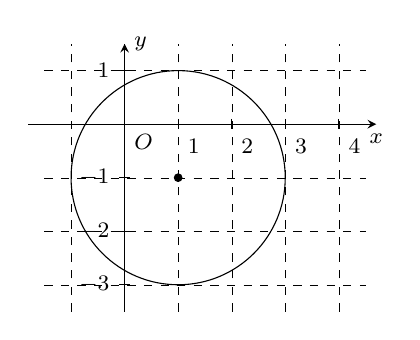
\begin{tikzpicture}[smooth,samples=300,scale=0.68,>=stealth,font=\footnotesize]
			\draw[line  width=0.1pt,dashed] (-1.5,-3.5) grid (4.5,1.5);
			\draw[->]  (-1.8,0)--(4.7,0) node[below]{$x$};
			 \draw[->] (0,-3.5)--(0,1.5) node[right]{$y$};
			\draw (0,0) node[below  right]{$O$};
			\draw (1,-1) circle  (2cm);
			\draw[fill=black] (1,-1) circle (2pt); 
			\foreach  \x in {1,2,3,4}\draw (\x,0.1)--(\x,-0.1) node [below right] {\footnotesize $\x$};
			\foreach \y in {-3,-2,-1,1}\draw (0.1,\y)--(-0.1,\y) node [left] {\footnotesize  $\y$};
		\end{tikzpicture}
	 }
	\loigiai{ 
		Đường tròn  có tâm $I(1;-1)$ và bán kính $R=2$ nên có dạng $(x-1)^2+(y+1)^2=4$.
	 }
\end{ex}

% nguồn: MaHoaNH_TuLuan_Lop10
\begin{bt}%[0H9Y4-2]%[ma:4ea01bed]
	Trong mặt phẳng tọa độ  $Oxy$, viết phương trình chính tắc của elip $(E)$ biết tiêu cự bằng $18$ và độ dài trục lớn bằng $24$.
	 \loigiai{
		Giả sử $(E)\colon \dfrac{x^2}{a^2}+\dfrac{y^2}{b^2} = 1$ là phương trình  elip cần tìm.\\
		Vì $(E)$ có tiêu cự bằng $18$ nên $2c=18$ suy ra $c=9$.\\ 
		Vì $(E)$ có độ dài trục lớn bằng $24$ nên $24=2a$ suy ra  $a=12$.\\
		Ta cũng  có $b=\sqrt{a^2-c^2}=3\sqrt{7}$.\\
		Vậy  $(E) \colon \dfrac{x^2}{144}+\dfrac{y^2}{63}=1$.
	} 
\end{bt}

% nguồn: MaHoaNH_TuLuan_Lop10
\begin{bt}%[0H9B4-2]%[0H9B2-2]%[0H9B3-2]%[ma:168cb71c]
	Trong  mặt phẳng $Oxy$, cho ba điểm $A(-5;0)$, $F(3;0)$, $M(1;-2)$.
	\begin{enumerate}[a)]
		\item Viết phương trình chính tắc của $(E)$ có một đỉnh là $A$  và nhận $F$ làm một tiêu điểm.
		\item Viết phương trình tổng quát của đường thẳng đi qua $M$ và vuông  góc với đường thẳng $d\colon 2x-y+1=0$.
		\item Viết phương trình đường tròn tâm $F$ và tiếp xúc với đường thẳng $AM$. 
	\end{enumerate}
	 \loigiai{
		\begin{enumerate}[a)]
			\item Gọi  phương trình chính tắc của $(E)$ có dạng $\dfrac{x^2}{a^2}+\dfrac{y^2}{b^2}=1$, $(0<b<a)$.\\
			Vì $(E)$ có một đỉnh là $A(-5;0)$ và nhận $F(3;0)$ làm một tiêu điểm nên $a=5$; $c=3$.\\ 
			Ta có $b^2=a^2-c^2=16$.\\ 
			Vậy phương trình chính tắc của  $(E)$ là $\dfrac{x^2}{25}+\dfrac{y^2}{16}=1$.
			\item Gọi $\Delta$ là đường thẳng đi qua $M$ và  vuông góc với đường thẳng $d\colon 2x-y+1=0$.\\
			$\Delta$ có  một véc-tơ pháp tuyến $\overrightarrow{n}_{\Delta}=(1;2)$.\\
			Phương trình tổng quát của  $\Delta$ là $1\cdot(x-1)+2\cdot(y+2)=0$ hay $\Delta\colon x+2y+3=0$.
			\item Gọi $(C)$ là đường tròn tâm $F$ và tiếp xúc  với đường thẳng $AM$, ta có $R=\mathrm{d}\left(F,AM\right)$ là bán kính của $(C)$.\\
			Ta có $\overrightarrow{AM}=(6;-2)$,  suy ra $\overrightarrow{n}=(1;3)$ là một véc-tơ pháp tuyến của $AM$.\\
			Phương trình đường thẳng $AM$ là $1\cdot(x+5)+3\cdot(y-0)=0$  hay $AM\colon x+3y+5=0$.\\
			Suy ra  $R=\mathrm{d}\left(F,AM\right)=\dfrac{\left|3+3\cdot 0+5\right|}{\sqrt{1^2+3^2}}=\dfrac{8}{\sqrt{10}}$.\\
			Vậy phương trình  đường tròn $(C)\colon (x-3)^2+y^2=\dfrac{32}{5}$.
		\end{enumerate}
	 }
\end{bt}
